\documentclass[flegn, 10pt]{report}
\usepackage[spanish]{babel}
\usepackage[utf8]{inputenc}
\usepackage{graphicx}
\usepackage[font=scriptsize]{caption}
\usepackage{amssymb,amsmath}
\usepackage{subfig}
\usepackage{float}
\usepackage{listings}
\usepackage[document]{ragged2e}
\usepackage[most]{tcolorbox}
\usepackage{hyperref}
\usepackage{csquotes}
\usepackage{geometry}
  \geometry{
    a4paper,
    total={170mm, 257mm},
    left=20mm,
    top=20mm,
  }
\hypersetup{
  colorlinks=true,
  urlcolor=blue,
}

\setlength{\parskip}{10px}
\definecolor{linequote}{RGB}{224,215,188}
\definecolor{backquote}{RGB}{249,245,233}

\newtcolorbox{myquote}{% Cuadro de referencia
  enhanced, breakable, 
  size=fbox,
  frame hidden, boxrule=0pt,
  sharp corners,
  colback=backquote,
  borderline horizontal={.5pt}{0pt}{linequote},
  borderline horizontal={.5pt}{1pt}{linequote}
}

\pagestyle{headings}

\begin{document}
  \begin{titlepage}
    \centering
    {
\includegraphics[width=0.8\textwidth]{unircol.png}\par}
    \vspace{1cm}
    {\bfseries\LARGE Fundación Universitaria Internacional De La Rioja \par}
    \vspace{1cm}
    {\scshape\Large PREGRADO DE INGENIERÍA INFORMÁTICA \par}
    \vspace{3cm}
    {\scshape\Huge Introducción a OpenGL \par}
    \vspace{3cm}
    {\itshape\Large Informática Gráfica y Visualización (COLGII) - Enero2022 \par}  
    \vfill
    {\Large Docente: \par}
    {\Large Rogerio Orlando Beltr\'an Castro \par}
    \vfill
    {\Large Autor: \par}
    {\Large Nicolás Zapata \'Alzate \par} 
    \vfill
    {\Large Abril de 2022 \par}
  \end{titlepage}

  \tableofcontents
  \newpage
  Cordial Saludo para el docente o quién tenga la autorización de revizar/calificar éste documento, como siempre, agradecido con Dios de poder estár vivo presentando éstos trabajos y poder seguir creciendo en la carrera de Ingeniería Informática.

Espero que el trabajo que estoy presentando cumpla con las pautas y pueda meritar una buena calificación.

El archivo está todo organizado en el apartado de la asignatura, en una carpeta llamada \textbf{<<app>>}. De igual manera, se encuentra anexado el link del repositorio de Github de éste mismo proyecto, tanto del proyecto (alojado en la carpeta app) como del proyecto del documento (alojado en la carpeta latex).







  \chapter{Herramientas utilizadas para el laboratorio} \label{chap:herramientas}
Para el desarrollo de éste laboratorio, hicimos uso de herramientas de desarrollo, en su mayoría, basadas para entornos Linux, ya que, he percatado de que tiene mejor rendimiento y mejores resultados que trabajar dentro del sistema operativo Windows.

\section{Entorno de desarrollo}
Se usaron las siguientes herramientas.

\begin{itemize}
\item WSL para Windows.
\item Python 3.
\item freegut-dev.
\item Neovm
\item Anaconda
\end{itemize}

\section{Organización del proyecto.}
\subsection{Librerías utilizadas.}
Como se mencionó en la anterior lista, he decidido presindir del lenguaje de programación Python para el desarrollo del laboratorio. Puesto que es un lenguaje en la que me he desempeñado en trabajar desde hace un buen tiempo desde que estudio en la universidad.

\begin{figure}[H]
\centering
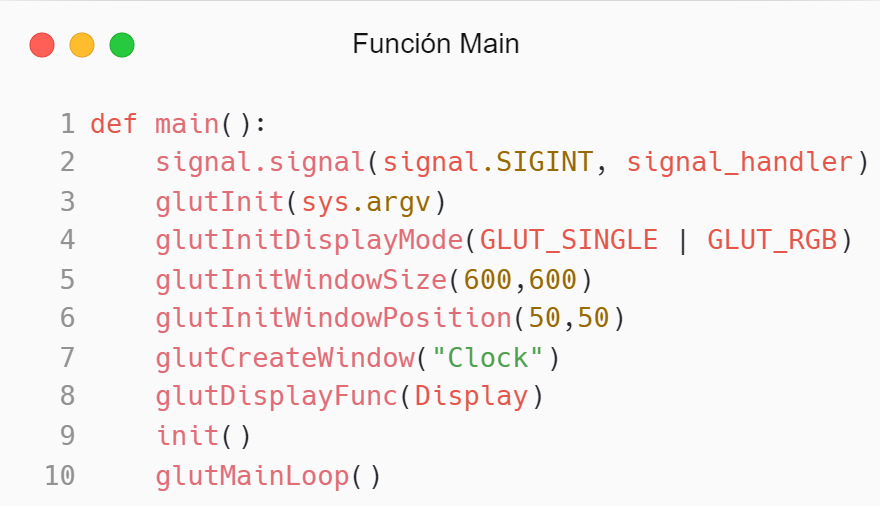
\includegraphics[width=0.4\textwidth]{../img/chapter01/1.png}
\caption{Librerías usadas para el laboratorio}
\label{fig:librerias_py}
\end{figure}

Las librerías más importantes para el laboratorio son las que vienen con PyOpenGL, que vienen con sus clases \textbf{GL, GLU y GLUT}, las cuales ejecutan las funciones y comamdos de OpenGL en Python.

En segundo lugar, tenemos la librería de \textbf{Time y Datatime} para el manejo del tiempo y de las fechas, nos ayuda a saber como está la hora y como ésta va repercutiéndose en el reloj.

Otra librería que no tiene mucho que ver con el uso de OpenGL, pero que, hace que sea más estilizado el programa, es la librería sys que, llama comandos de la terminal, como por ejemplo, limpiar la consola, realizar o llamar comandos, entre otras acciones que hacemos dentro de la terminal, y que en Python nos ayuda a ejecutar dentro del programa.

\subsection{Árbol del proyecto.} \label{subsec:arbol}
El archivo en general cuenta con una clase main que es la principal, contamos con una carpeta llamada \textbf{components}, en donde están los archivos \textbf{clock, display y draw}, la primera, es la clase en donde está trabajada las funciones que tienen que ver con la organización del reloj, la clase display, es la clase en donde se encuentra el método para la iniciación de la ventana, que es la gui en donde se visualiza el reloj, por último, está la clase draw, en donde están los métodos en donde se hace la manipulación de los elementos del reloj.

\begin{figure}[H]
	\centering
	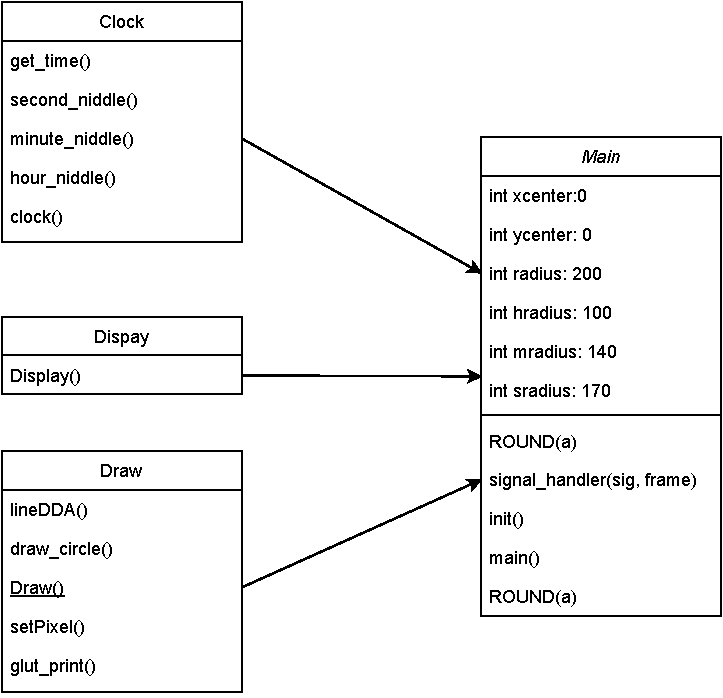
\includegraphics[width=0.8\textwidth]{../img/chapter02/3.pdf}
	\caption{Diagrama de clases del proyecto.}
	\label{fig:diagrama_clases}
\end{figure}








  \chapter{Decripción del código} \label{chap:descripcion_codigo}
\section{Clase Main.} \label{sec:main}
\section{Variables de iniciación} \label{subsec:variables}
las variables que se usaron, son las variables que definen la lógica del programa.

\begin{figure}[H]
\centering
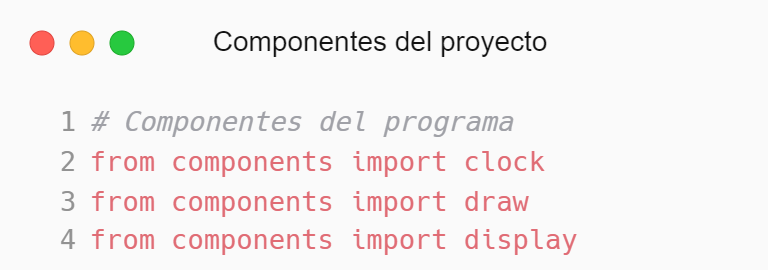
\includegraphics[width=0.4\textwidth]{../img/chapter02/2.png}
\caption{Varibles inicializadas}
\label{fig:variables_iniciales}
\end{figure}

Como se observa en la figura \ref{fig:variables_iniciales}, están los ejes \textbf{x} y \textbf{y}, Tenemos los radios del círculo para éste caso, los cuales están los respectivos radios para las manecillas del reloj (segundo definido con valor 200, minuto 100 y hora 170).

\subsection{Clase Clock.} \label{subsec:clock}
Como se explicón en el apartado \ref{subsec:arbol}, conversamos de una clase que tiene que los métodos que trabajan con las animaciones que simula un reloj andando (que no es algo obligatorio para el laboratorio, es un extra que trae el proyecto que edité).

\begin{figure}[H]
	\centering
	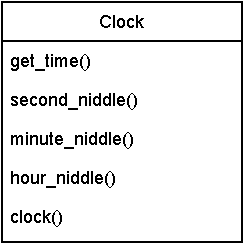
\includegraphics[width=0.4\textwidth]{../img/chapter02/4.pdf}
	\caption{Clase Clock}
	\label{fig:clock}
\end{figure}

Ésta clase, como se muestra en la figura \ref{fig:clock}, tiene los métodos \textbf{get\_time, second\_niddle, minute\_niddle, hour\_niddle y clock}.

\subsection{Clase Display.} \label{subsec:display}
Ésta clase sólo tiene un método que es, irónicamente, un método que tiene el mismo nombre que la clase

\begin{figure}[H]
	\centering
	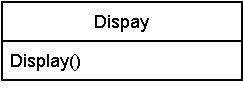
\includegraphics[width=0.4\textwidth]{../img/chapter02/5.pdf}
	\caption{Clase Clock}
	\label{fig:clock}
\end{figure}

La función de la ésta clase, maneja la posición, el tamaño, y demás items de las ventanas visuales del programa.

\subsection{Clase Draw.} \label{subsec:draw}

Ésta clase contiene los métodos lineDDA, draw\_circle, draw, setPixel y glutPrint.

\begin{figure}[H]
	\centering
	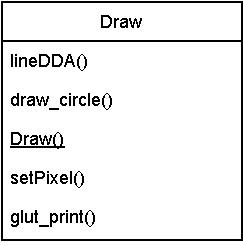
\includegraphics[width=0.2\textwidth]{../img/chapter02/6.pdf}
	\caption{Clase Clock}
	\label{fig:clock}
\end{figure}






  \chapter{conclusiones} \label{Conclusiones}

\section{Resultados y pautas de la actividad.} \label{sec:resultado}
\subsection{Resultado.} \label{subsec:resultado}
Éste es el resultado del proyecto editado.

\begin{figure}[H]
\centering
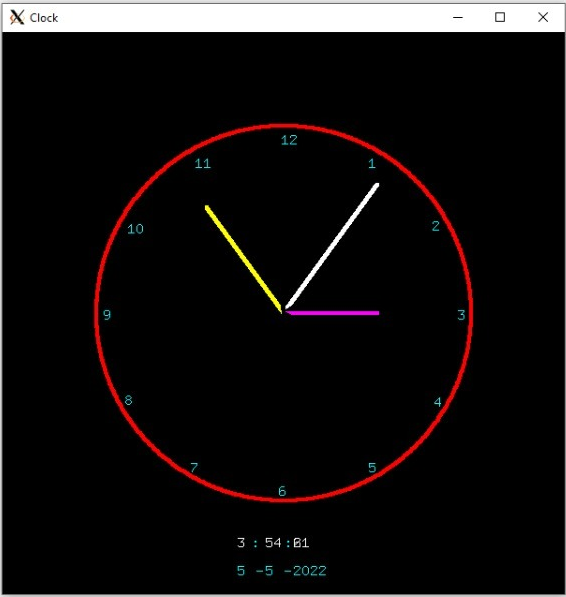
\includegraphics[width=0.4\textwidth]{../img/chapter03/7.png}
\caption{Resultado del proyecto}
\label{fig:resultado}
\end{figure}

La diferencia que se puede ver aquí,es que, ya que WSL (por lo menos en su versión 1) no tiene capacidad de ejecutar gui nativamente, por lo que tuve que usar un servidor para que pudiera correr la gui de la aplicación desde WSL.

\subsection{Pautas del ejercicio.} \label{subsec:pautas}
Luego de lo mostrado alrededor de los capítulos, y de ilustrar el resultado obtenido en el apartado \ref{subsec:resultado}, vamos a disponer de responder unas pautas que nos deja el ejercicio.

\begin{myquote}
¿Funciona bien tu programa?
\end{myquote}

como vimos en la figura \ref{fig:resultado}, el reloj funciona correctamente.

\begin{myquote}
¿Qué fallos existen?
\end{myquote}

Como tal, no se encontraro errores en la primera versión del archivo donde no hace uso de la programación orientada a objetos, sin embargo, por la dificultad de poder visualizar el resultado por mí mismo (porque el proceso es muy lento por el uso de XLaunch para windows, la primera versión me la revizó un compañero de la universidad, a quién nombraré en el apartado de agradecimientos).

\chapter{Recursos}
\href{https://pharos.sh/breve-introduccion-a-opengl-en-python-con-pyopengl/}{https://pharos.sh/breve-introduccion-a-opengl-en-python-con-pyopengl/}

\href{https://codingshiksha.com/python/python-3-opengl-script-to-build-3d-digital-analog-clock-using-pyopengl-library-gui-desktop-app-full-project-for-beginners/}{https://codingshiksha.com/python/python-3-opengl-script-to-build-3d-digital-analog-clock-using-pyopengl-library-gui-desktop-app-full-project-for-beginners/}

\href{https://yewtu.be/watch?v=9rmxMUyFcj4}{https://yewtu.be/watch?v=9rmxMUyFcj4}



\chapter{Agradecimientos}
Mi especial agradecimiento a mi compañero \textbf{Sebastian Steffen Castañeda Castillo} por la ayuda y colaboración para ayudarme a comprobar el funcionamiento del proyecto debido que a causas técnicas, no pude comprobarlos por mí mismo.

De igual manera, agradecer a todos aquellos compañeros que, de forma desinteresada, me han aportado con sus conocimientos el poder llevar adelante éste laboratorio.




\end{document}
